\documentclass[tikz]{standalone}

\usepackage{tikz}
\usetikzlibrary{positioning, arrows.meta, shapes, snakes, shadings}
\usepackage{amsmath,amssymb,amsthm,pgfplots}

\pgfmathdeclarefunction{gauss}{2}{%
  \pgfmathparse{1/(#2*sqrt(2*pi))*exp(-((x-#1)^2)/(2*#2^2))}
}

% polychrome colour, kelly
\definecolor{kwhite}{RGB}{242,243,244}
\definecolor{kred}{RGB}{175,35,55}
\definecolor{kyellow}{RGB}{236,195,66}
\definecolor{kblue}{RGB}{41,103,160}
\definecolor{kolivegreen}{RGB}{47,60,40}
\definecolor{kyellowgreen}{RGB}{150,180,55}
\definecolor{kpurplishpink}{RGB}{218,147,171}
\definecolor{korange}{RGB}{229,137,50}
\definecolor{kpurple}{RGB}{128,89,143}
\definecolor{kreddishbrown}{RGB}{126,51,31}
\definecolor{kgreen}{RGB}{59,133,90}
\definecolor{kbuff}{RGB}{192,178,134}
\definecolor{klightblue}{RGB}{169,201,237}
\definecolor{kyellowishpink}{RGB}{236,151,127}
\definecolor{kgrey}{RGB}{132,132,130}
\definecolor{kyellowishbrown}{RGB}{96,70,40}
\definecolor{kreddishorange}{RGB}{210,96,52}
\definecolor{kpurplishred}{RGB}{166,76,107}
\definecolor{kgreenishyellow}{RGB}{219,210,69}
\definecolor{korangeyellow}{RGB}{235,168,59}
\definecolor{kviolet}{RGB}{93,80,146}
\definecolor{kblack}{RGB}{34,34,34}
\definecolor{eedarkblue}{HTML}{202040}
\definecolor{eepurple}{HTML}{543864}
\definecolor{eered}{HTML}{ff6363}
\definecolor{eeyellow}{HTML}{ffbd69}
\definecolor{eecyan}{HTML}{64ccda}

\begin{document}
    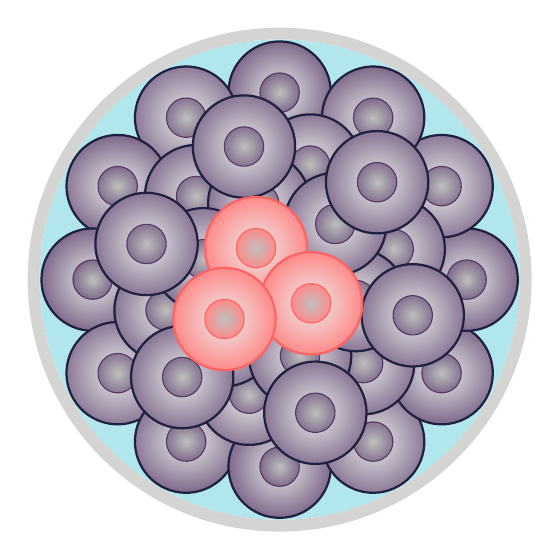
\begin{tikzpicture}
        % background
        \draw[draw=none, fill=eecyan!50] (3,3) circle[radius=3.05];
        
        % outer blastomeres
        \foreach \x in {0,30,60,...,330}
        {
            \draw[thick, draw=eedarkblue, inner color=gray!15, outer color=eepurple!75, rotate around={\x:(3,3)}] (3,5.375) circle[radius=0.65];
            \draw[draw=eepurple, inner color=gray!50, outer color=eepurple!75, rotate around={\x:(3,3)}] (3,5.375) circle[radius=0.25];
        }
        % inner blastomeres
        \foreach \x in {45,105,165,225,285,345}
        {
            \draw[thick, draw=eedarkblue, inner color=gray!15, outer color=eepurple!75, rotate around={\x:(3,3)}] (3,4.5) circle[radius=0.65];
            \draw[draw=eepurple, inner color=gray!50, outer color=eepurple!75, rotate around={\x:(3,3)}] (3,4.5) circle[radius=0.25];
        }
        % inner blastomeres
        \foreach \x in {15,75,...,315}
        {
            \draw[thick, draw=eedarkblue, inner color=gray!15, outer color=eepurple!75, rotate around={\x:(3,3)}] (3,4) circle[radius=0.65];
            \draw[draw=eepurple, inner color=gray!50, outer color=eepurple!75, rotate around={\x:(3,3)}] (3,4) circle[radius=0.25];
        }
        % fill in the gaps
        \foreach \x in {15,75,135,195,255,315}
        {
            \draw[thick, draw=eedarkblue, inner color=gray!15, outer color=eepurple!75, rotate around={\x:(3,3)}] (3,4.75) circle[radius=0.65];
            \draw[draw=eepurple, inner color=gray!50, outer color=eepurple!75, rotate around={\x:(3,3)}] (3,4.75) circle[radius=0.25];
        }
        % pluripotent cells
        \draw[thick, draw=eered, inner color=gray!15, outer color=eered!75] (2.7,3.4) circle[radius=0.65];
        \draw[eered, inner color=gray!50, outer color=eered!75] (2.7,3.4) circle[radius=0.25];
        \draw[thick, draw=eered, inner color=gray!15, outer color=eered!75] (3.4,2.7) circle[radius=0.65];
        \draw[eered, inner color=gray!50, outer color=eered!75] (3.4,2.7) circle[radius=0.25];
        \draw[thick, draw=eered, inner color=gray!15, outer color=eered!75] (2.3,2.5) circle[radius=0.65];
        \draw[eered, inner color=gray!50, outer color=eered!75] (2.3,2.5) circle[radius=0.25];
       
        % zona pellucida
        \draw[draw=none, fill=kgrey!35, even odd rule]
            (3,3) circle[radius=3.2] (3,3) circle[radius=3.05];
        
%        \draw[help lines, step=0.1] grid(6,6);
    \end{tikzpicture}   
\end{document}